\documentclass[border=10pt]{standalone}

\usepackage{tikz}
\usepackage{tikzsymbols}
\usetikzlibrary{calc,patterns,shapes.geometric}

\def\centerarc[#1](#2)(#3:#4:#5){\draw[#1] ($(#2)+({#5*cos(#3)},{#5*sin(#3)})$) arc (#3:#4:#5);}

\begin{document}
	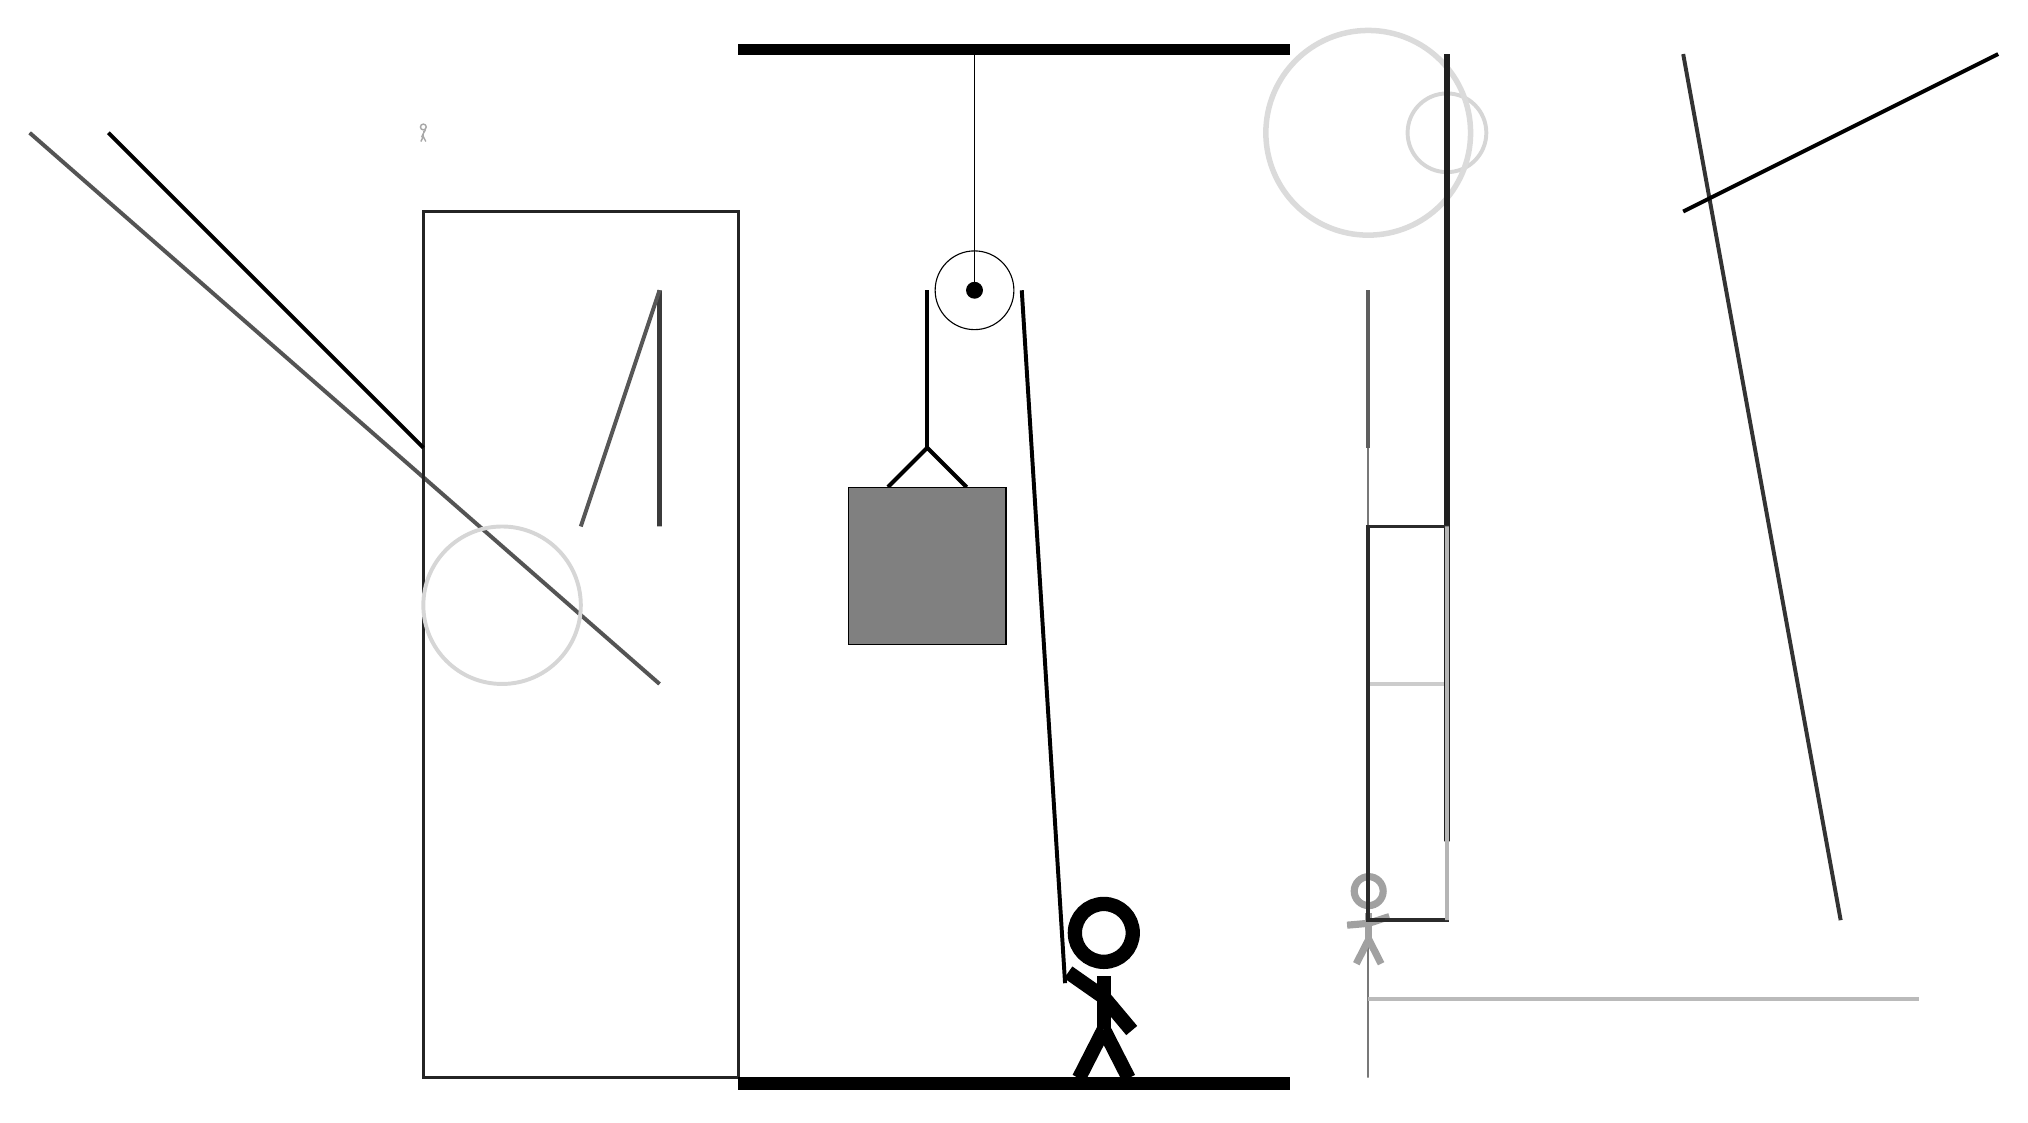
\begin{tikzpicture}
		%%%%% START %%%%%
		
		\draw[fill=black] (-2, 10) rectangle (5, 10.125);
		
		\draw (1, 7) circle (0.5);
		\draw[fill=black] (1, 7) circle (0.1);
		\draw (1, 10) -- (1, 7);
		
		\draw[line width=0.6mm, color=black!77] (-3, 4) rectangle (-3, 7);
		
		\draw [line width=0.5mm, color=black!16](7, 9) circle (0.5);
		\draw[line width=0.5mm, color=black!67](-3, 2) -- (-11, 9);
		\draw[line width=0.3mm, color=black!53] (6, -3) rectangle (6, 5);
		\draw [line width=0.7mm, color=black!14](6, 9) circle (1.3);
		\draw[line width=0.4mm, color=black!86] (-2, 8) rectangle (-6, -3);
		\draw[line width=0.4mm, color=black!20] (6, -1) rectangle (7, 2);
		\draw[line width=0.7mm, color=black!88] (7, 10) rectangle (7, 0);
		\draw[line width=0.5mm, color=black!80](10, 10) -- (12, -1);
		\node[line width=0.2mm, color=black!37] at (6, -1) {\Strichmaxerl[5][5][18]};
		
		\draw[line width=0.5mm, color=black!63](6, 5) -- (6, 7);
		
		\draw[line width=0.5mm, color=black!83] (6, -1) rectangle (7, 4);
		\node[line width=0.7mm, color=black!34] at (-6, 9) {\Strichmaxerl[1][66][60]};
		
		\draw[line width=0.5mm, color=black!27](6, -2) -- (13, -2);
		\draw[line width=0.6mm, color=black!29] (7, 4) rectangle (7, -1);
		\draw[line width=0.5mm, color=black!100](-6, 5) -- (-10, 9);
		\draw[line width=0.5mm, color=black!100](10, 8) -- (14, 10);
		\draw[line width=0.5mm, color=black!66](-3, 7) -- (-4, 4);
		\draw [line width=0.5mm, color=black!16](-5, 3) circle (1.0);
		
		\draw[line width=0.5mm] (-0.1, 4.5) -- (0.4, 5.0) -- (0.9, 4.5);
		\draw[fill=black!50] (-0.6, 4.5) rectangle (1.4, 2.5);
		
		\draw[line width=0.5mm] (0.4, 7) -- (0.4, 5.0);
		\centerarc[line width=0.5mm](1, 7)(0:180:0.6);
		\draw[line width=0.5mm](1.6, 7) -- (2.15, -1.8);
		
		\node at (2.6, -1.9) {\Strichmaxerl[10][-35][-50]};
		
		\draw[fill=black] (-2, -3) rectangle (5, -3.15);
		
		%%%%% END %%%%%
	\end{tikzpicture}
\end{document}